\chapter{Work Package Tasks}
\label{ch:wptasks}

In this chapter, the high level tasks in each WP is discussed briefly. A reference architecture diagram is also given for each WP, this is meant to be seen as an early proposal and it is subjected to change in future documents.

\section{WP1: Service Descriptor Translator}

\subsection{Requirements definitions and architecture design}
\paragraph{}
The development of the SDT engine follows a microservice architecture. The architecture inludes a message broker with a publish/subcribe model. The NSDs(yaml files) corresponding to the communicating MANO are published to the broker. Our SDT engine, subscribed to the broker, consumes the yaml files and translate one MANO NSD to the other template and publish them back to the broker. These translated NSDs could be accessed by any other services through a REST API.
\begin{figure}[h]
	\centering
	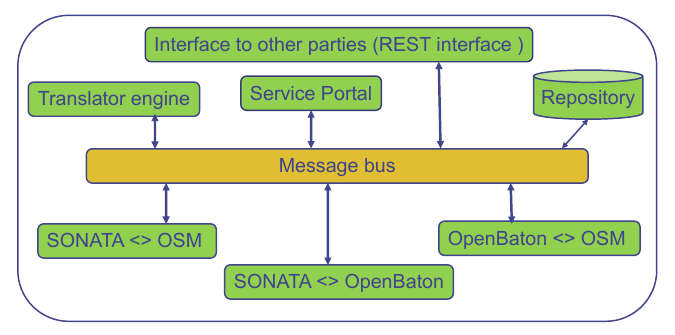
\includegraphics[width=0.9\linewidth]{figures/wp1Arch}
	\caption{Reference architecture for SDT \cite{WPDescriptionsPDF}}
	\label{fig:wp1arch}
\end{figure}

\subsection{Prototype implementation of SDT components}
\paragraph{}
After the concrete architecture is planned, a working prototype of the SDT engine including all the requisite components is modeled. This prototype is built as a standalone autonomous microservice.
\subsection{Proof of concept demonstration}
\paragraph{}
The functionality of the SDT engine will be demonstrated on virtual machines containing atleast two different MANO frameworks installed and deployed. 

\section{WP2: Service Descriptor Splitter}

\subsection{Requirements definition and architecture design}
\paragraph{}
  A publish/subscribe message broker model will be once again followed for the SDS engine implementation. The NSD(yaml file) is published to the message broker. A service graph splitter and a NSD splitter consumes the NSD from the broker and splits the NSD into two. The two seperate NSDs are published back to the broker from where other services can consume those through REST API.
\begin{figure}[h]
	\centering
	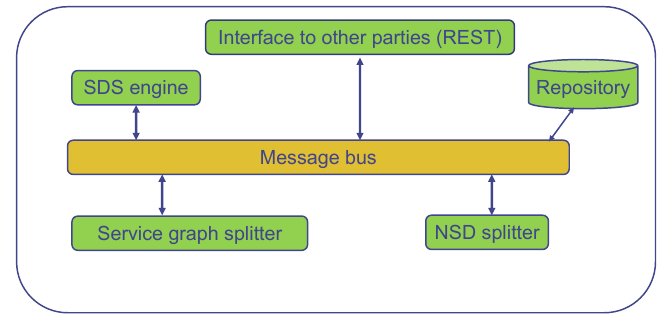
\includegraphics[width=0.9\linewidth]{figures/wp2Arch}
	\caption{Reference architecture for SDS \cite{WPDescriptionsPDF}}
	\label{fig:wp2arch}
\end{figure}

\subsection{Investigation of service graph partitioning algorithms and libraries}
\paragraph{}
The service graph needs to be split optimally based on the loads and resource allocation on each VNF. To accomplish this a graph partitioning algorithm such as \textit{Mixed Integer Program for Partitioning Graphs} \ref{MIPPG} will be used. However the exact choice of algorithm suitable for the project will be decided going forward.
\subsection{Prototype implementation of SDS components}
\paragraph{}
After the concrete architecture is planned, a working prototype of the SDS engine including all the requisite internal components is coded and modeled. This prototype is also built as a standalone autonomous microservice.
\subsection{Proof of concept demonstration}
\paragraph{}
The functionality of the SDS engine will be demonstrated on virtual machines containing atleast two different MANO frameworks installed and deployed. 

\section{WP3: MANO Adaptor}

\subsection{Requirements definition and architecture design}
\paragraph{}

\begin{figure}[h]
	\centering
	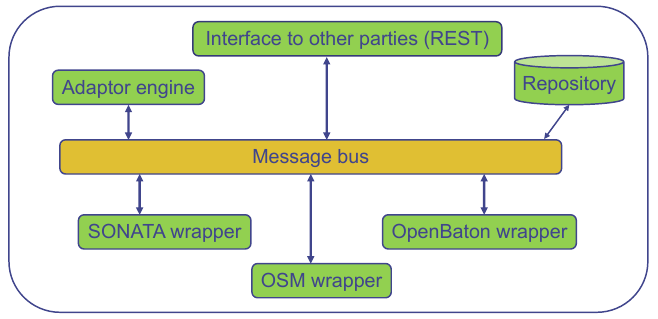
\includegraphics[width=0.9\linewidth]{figures/wp3Arch}
	\caption{Reference architecture for MA \cite{WPDescriptionsPDF}}
	\label{fig:wp3arch}
\end{figure}

\subsection{Prototype implementation of adaptor components}
\paragraph{}
As a starting point of the prototype, the plan is to choose one of the MANO frameworks listed in the section \ref{manoframeworks} and implement the wrapper for the interfaces provided by it, with focus on modularity and portability. Thereby, making it easy to add support for interfaces provided by other MANO frameworks. Further, we will add the southbound interfaces required to communicate with the MA.

\subsection{Investigation of MANO scalability challenges}
\label{wp3manoresearch}
The plan is to investigate MANO scalability challenges by answering research questions such as the ones listed below but not limited to. (Figure \ref{fig:wp3manoscale})
\begin{itemize}
	\item What is the optimal number of MANO instances in a system?
	\item What is the optimal hierarchical level in a system?
\end{itemize}

\begin{figure}[h]
	\centering
	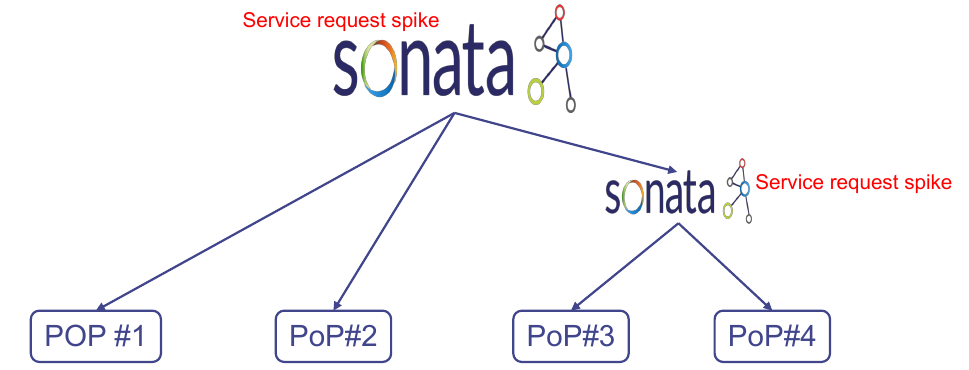
\includegraphics[width=0.9\linewidth]{figures/wp3manoScale}
	\caption{MANO scaling scenario \cite{WPDescriptionsPDF}}
	\label{fig:wp3manoscale}
\end{figure}


\subsection{Proof of concept demonstration}
MA is demonstrated by having two/three virtual machines with MANO frameworks installed, a scenario where a huge number of service requests on one of the MANOs is created. In order to balance the load, the MANO experiencing the service request spike splits the load with another MANO instance. The capability of the MANO to communicate between other MANO instances with the help of MA is thus demonstrated.
